
\documentclass{article}

\usepackage{p200}
\usepackage[colorlinks=true,linkcolor=blue]{hyperref}

\hypersetup{pdftitle = {Physics 203 } }
\hypersetup{pdfauthor = {}, pdfsubject = {Physics} }

\pagestyle{headings}

\begin{document}

\setcounter{page}{1}

\begin{tikzpicture}[remember picture,overlay]
\node [xshift=-1in,yshift=-1in] at (current page.north east) [below left] {Name: \underline{\makebox[2in]{}}};
\end{tikzpicture}

\begin{center}
\LARGE{Physics 203 Quiz 1} \\[2mm]
\small{\sf Jun 26, 2013}
\end{center}

\thispagestyle{empty}

\section*{Word Problems}
Show all your work and circle your final answer. (Ten points each.) \par


\textbf{1.} \quad An evil genius wants to shrink the Moon in order to steal it. He
accidentally shrinks its below it Schwarzschild radius and the Moon
is lost forever in a mini-black hole. What is this radius?


\begin{center}
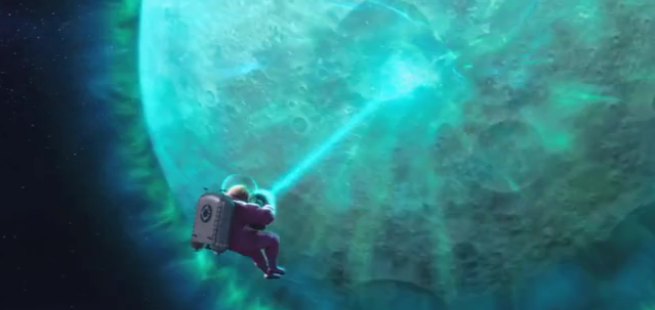
\includegraphics[scale=0.4]{C:/"Program Files"/my/github/spot/content/images/gru-shrinks-moon2.png}

\label{fig:gru-shrinks-moon2-png}
\end{center}
\par {\footnotesize\sf Answer: 0.109 millimeters}
\par We simply use the definition of the Schwarzschild radius:
%
\begin{equation*}
r_s = \frac{2GM}{c^2}
\end{equation*}
The $GM$ value for the moon is
%
\begin{equation*}
GM = (\sci{6.673}{-11})(\sci{7.36}{22})
= \sci{4.9113}{12}
\end{equation*}
So...
%
\begin{equation*}
r_s = \frac{(2)(\sci{4.9113}{12})}{(\sci{2.998}{8})^2}
= \sci{1.0929}{-4}
\end{equation*}
\newpage

\textbf{2.} \quad A certain mass spectrometer is designed with a radius of 0.40 meters using a magnetic field of 2.0 tesla. What electric voltage is required to accelerate a doubly ionized ozone molecule to travel through the spectrometer?
\par {\footnotesize\sf Answer: TBD}
\par No solution available.
\newpage


\end{document}